\subsection*{Leveling determination of the geopotential difference}

The static gravitational-redshift correction is fixed by the
geopotential difference between the atomic-transition positions of the
two clocks, determined by a first-order spirit leveling campaign
carried out specifically for this comparison: a
$\levelKm$\,km line between the Wuhan benchmark WS-03 and the
Shanghai benchmark WS-01, observed in both directions with digital
levels and bar-code invar staffs, with gravity observed along the
line. The geopotential difference is integrated section by section,
$\dW_{AB} = -\sum_i g_i\,\Delta H_i$, and combined with the local
benchmark-to-transition offsets, giving
$\dW = \dWVal \pm \dWUnc~\mathrm{m^2\,s^{-2}}$, equivalent to an
optical fractional shift of $\deltaGV$. The per-kilometer accidental
error $M_\Delta = \levelMm$\,mm\,km$^{-1}$ satisfies the most
stringent first-order requirements of the Chinese, US, German and
Czech national standards (Supplementary
Section~3)~\citep{fgcc1984,gb12897,cuzk2015,advfapn2022}. An
independent GNSS-plus-EGM2008 geoid-model calibration gives
$\dWAlt \pm \dWAltUnc~\mathrm{m^2\,s^{-2}}$, consistent with the
leveled value but about 30 times less precise, so it serves as a
consistency check rather than a calibration at the reported
accuracy.

\subsection*{Experimental setup, frequency transfer and data processing}

The two sites are connected by a phase-stabilized fiber link of
$\fibreKm$\,km single-pass length ($\roundKm$\,km loop-back),
operated at \qty{1550}{nm} and carried on a commercial telecom
network used non-exclusively. The route is divided into spans of tens
of kilometers, each terminated by a relay station carrying a
narrow-linewidth laser, an erbium-doped fiber amplifier and a
fiber-noise-cancellation loop; the added instability of the link is
kept below the clock noise for averaging times beyond $100$\,s.

Both ends use independent optical frequency combs, self-referenced
and phase-locked to their local clock, to bridge the spectral gap
between the clock transitions and the telecom carrier; all frequencies
in the chain derive from the two clock transitions through fixed
factor-of-two relations, $f_{\mathrm{comb}}^{1397} =
\tfrac{1}{2}(1+a)\,f_{\mathrm{Sr}}$ and $f_{\mathrm{comb}}^{1156} =
\tfrac{1}{2}(1+b)\,f_{\mathrm{Yb}}$, where $a$ and $b$ collect the Sr
and Yb systematic corrections (density, lattice, second-order Zeeman
and blackbody shifts). The observable is the
out-of-loop beat between the received carrier and the local
Yb-referenced comb, converted to fractional units with the transfer
frequency $f_{1550} = \fFifteenTHz$\,THz. The static
gravitational-redshift correction enters the ratio inversion as a
multiplicative factor,
$\left(\mathrm{Yb/Sr}\right)_{\rm corr}
= \left(\mathrm{Yb/Sr}\right)_{\rm raw} \times (1+\delta_g)$ with
$\delta_g = \deltaGV$, derived from the leveled geopotential
difference above.

The counters sample the beat every second in phase-averaging mode.
Each accepted segment contributes its longest jump-free record; the
per-segment retained counts, ratio deviations and statistical
uncertainties are listed in Supplementary Table~1. Five segments
whose stability slopes fall outside the white-frequency-noise band
are flagged there as model-limited; they lie at the steep end of a
continuous slope distribution with no common campaign, weather or
laboratory condition that distinguishes them from the remaining
segments.

\subsection*{Tidal analysis}

Two analyses quantify the tidal impact on the ratio, each with its
own quantity: the within-segment response of the beat waveform
(Section~\ref{sec:results-budget} of the main text) and the spliced
stability of the concatenated record (below). They are equivalent
measures of the same effect---how strongly the beat follows the tidal
template---and are expected to converge as the record grows; we
report both.

\emph{Tidal templates and the correction test.} The solid Earth tide
and ocean tide loading displacement difference between the two sites
is computed every \qty{30}{s} with the public software
ETideLoad4.5, converted to an equivalent geopotential difference and
then to a beat-frequency template $h = f_{1550}\,\Delta W/c^2$ with
the same $f_{1550}$ normalization as the beat record. A second,
independent template is built from the DE421 ephemerides and the
FES2022 ocean-tide model on a \qty{90}{s} grid. The within-segment
analysis windows the retained beat record and the 1-s template with
the same 1200-s triangular window at 600-s stride, demeans both, and
fits $\mathrm{beat} = A\cdot\mathrm{tide}$ through the origin, with
the template sign corrected for the beat polarity so that a positive
amplitude corresponds to the expected response $A = +1$; amplitudes,
Pearson $r$ and $p$ values are inferred from non-overlapping 1200-s
windows only, and the per-segment amplitudes are combined with
precision weights $1/u_A^2$. The combined response amplitudes are
$\tidalAmpOldE$ (ETideLoad4.5) and $\tidalAmpNewE$
(DE421+FES2022), as reported in the main text; because the two models
share the same beat record, their significance values are not
independent replications.

As a correction test, the ratio combination is repeated with the tide
series applied before the inversion at two fixed amplitudes, the
theoretical $A = +1$ and the historical $A = +0.54$ from the demeaned
beat waveform of our earlier analysis of the same campaign. Both
templates degrade rather than improve the fit: the reduced chi-square
of the combination rises from \tidalChiRaw~to \tidalChiTheory~and
\tidalChiEmp~for the ETideLoad4.5 template (Bayesian center shift
$-\tidalShiftEmpE\times10^{-18}$), and to \tidalChiAlt~for the
DE421+FES2022 template, which moves the center in the opposite
direction, by $+\tidalShiftAltE\times10^{-18}$. Repeating the
segment-mean correlation with the solid tide alone
($r = \tidalCorrSolid$ instead of \tidalCorrTotal) locates the
dominant coupling in the ocean-tide loading term. Templates that
degrade the segment agreement, and whose two independent realizations
disagree in sign, are treated as inconsistent with the data: no tidal
correction is applied to the reported central value, and the larger of
the two center shifts is carried as the time-varying-redshift
uncertainty item $\uTidalE\times10^{-18}$.

\emph{Spliced stability.} The \nSeg~segments were spliced end-to-end
on a continuous 1-s clock with the wall-clock gaps removed, giving a
single \nSamples~sample record whose overlapping Allan deviation
$\sigma_y(\tau)$ can reach averaging times beyond a single segment
(Figure~\ref{fig:spliced}). The spliced curve extends the
per-segment stability points to $\tau$ up to about 4.6 days of pure
data time, at which the raw record reaches
$\sigma_y \approx 8.6\times10^{-19}$; applying the two theoretical
tide corrections ($A = +1$) shifts the long-$\tau$ level by less than
$10\%$ in opposite senses, and the removed correction terms
($h/f_{1550}$) themselves lie below the corrected curves. Because the
spliced axis removes the inter-segment gaps, points with $\tau$
exceeding one segment mix different campaigns; the pair count behind
each point is reported with the data. This diagnostic is a data
record, not a statistical uncertainty.

\begin{figure}[t]
  \centering
  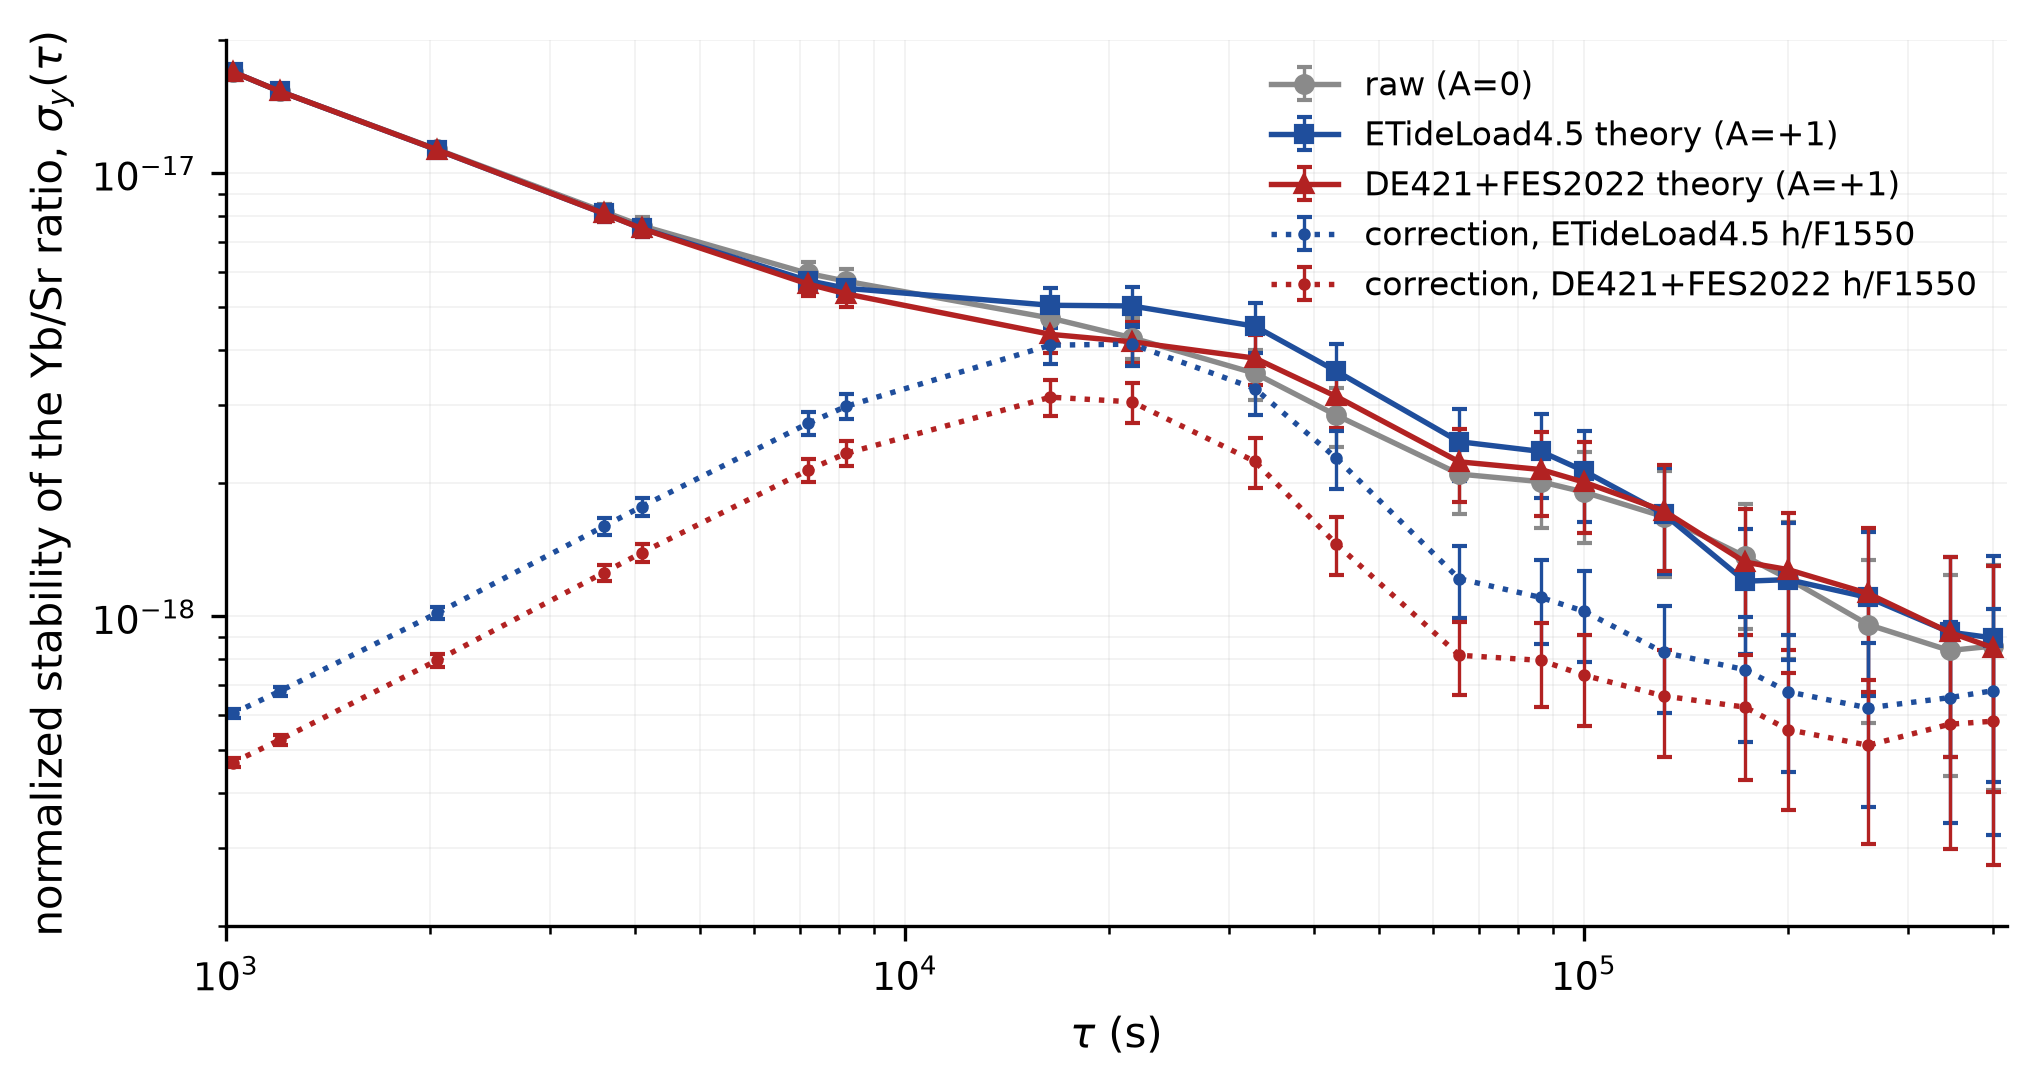
\includegraphics[width=\linewidth]{figs/fig5_spliced_stability.png}
  \caption{Spliced concatenated stability of the \nSeg~segments.
  The segments are placed end-to-end on a continuous 1-s clock (gaps
  removed, $\nSamples$ samples, \qty{11.4}{d} of pure data time); one
  overlapping Allan deviation per series, from $\tau = \qty{1000}{s}$
  to $\qty{4.6}{d}$. Curves: the raw record ($A=0$), the theoretical
  tide correction ($A=+1$) for the ETideLoad4.5 and DE421+FES2022
  templates, and the removed correction terms $h/f_{1550}$
  themselves (dotted). Error bars are 1-$\sigma$ equivalent degrees of
  freedom; the pair count at each $\tau$ is reported with the data.
  Points beyond one segment mix campaigns, so the curve is a data
  record rather than an uncertainty estimate.}
  \label{fig:spliced}
\end{figure}

The components of the uncertainty budget (Table~\ref{tab:budget})
are treated as independent and combined in quadrature, giving the
total standard uncertainty $\uTotalE \times 10^{-18}$.
